\documentclass[floats,floatfix,showpacs,amssymb,prd,superscriptaddress,nofootinbib]{revtex4-2} % documentation at https://journals.aps.org/revtex/revtex-faq#u2
\bibliographystyle{apsrev}

% \documentclass{article}
\usepackage[utf8]{inputenc}
\usepackage{graphicx}
\usepackage{wrapfig}
\usepackage{amsmath}
\usepackage{caption}
\usepackage{subcaption}
\usepackage{float}
\usepackage{hyperref}
\usepackage{xparse}
\usepackage[backend=biber]{biblatex}
\addbibresource{references.bib}
\usepackage{minted}
\usepackage{xcolor}
\definecolor{LightGray}{gray}{0.9}
\usepackage[left=2.54cm,right=2.54cm,top=2.54cm,bottom=2.54cm]{geometry}
\font\titlefont=cmr12 at 16pt
% inserting cover sheet: https://tex.stackexchange.com/questions/438775/how-to-insert-a-pdf-page-as-a-front-cover

% \newcommand{\PL}[1]{\textsf{\color{green!80!black}{\textsuperscript{PL}#1}}}
\newcommand{\code}{\texttt}
\setlength{\parindent}{20pt}
% \setstretch{1.25}

% \begin{figure}
%     \centering
%     \includegraphics[width=0.9\columnwidth]{images/Kyle_BLvsCR.png}
%     \caption{Recovered binary neutron star tidal parameters with and without binary Love relations, as compared to the common radius approximation.}
%     \label{fig:BLvsCR}
% \end{figure}

\begin{document}

\title{{\titlefont Effects of variable resolution and cosmological parameters
\\on the hydrogen 21cm cosmic dawn signal}\\{\small Supervised by Prof. Anastasia Fialkov and Jiten Dhandha}}
% project title : Impact of structure formation and cosmology on the hydrogen 21-cm signal from cosmic dawn
\date{9 December, 2024}
\author{Kyle Wong}
\affiliation{Institute of Astronomy, University of Cambridge, Madingley Road, Cambridge, CB3 0HA, UK}

% \begin{abstract}
% Summarize the problem we are solving and our main findings.
% \end{abstract}

\maketitle
\section{Introduction}
% As the simplest atom, hydrogen is of significant importance to 21st century astrophysicists. 

Because of its overwhelming dominance over other elements in its abundance, mapping the distribution of atomic hydrogen has the ability to inform the processes of structure formation, as well as shed light on the processes and events which occurred during the cosmic Dark Ages and Epoch of Reionization -- a period spanning between 375,000 years and 1 billion years after the big bang \cite{Pritchard_2012}. Conveniently, hydrogen occasionally emits photons of wavelength 21cm, resulting in the aptly named field of 21cm cosmology.

% Conveniently, hydrogen occasionally emits photons, which can be measured from Earth. This emission is produced by a spin-flip transition -- if the atom first starts with its proton's spin and electron's spin aligned, the electron sometimes spontaneously flips so that its spin is anti-aligned with the protons. This results in a photon of wavelength 21cm, and hence the aptly named field of 21cm cosmology.

% Combined with physical data such as those taken by the HERA, CHIME, and REACH, the simulations have the power to place constraints on viable theories.

The 21cm signal is of such importance that numerous simulations have been written to predict its signal. One such simulation, named \code{21cmSPACE}\footnote{This name, which stands for 21-cm Semi-numerical Predictions Across Cosmic Epochs, was not given until mid-2023; older papers referring to this code do not include this name.} \cite{Fialkov_2014}, has been developed by the Cambridge Cosmic Dawn group and uses a semi-numerical approach to achieve balance between accuracy and efficiency. At the basic level, \code{21cmSPACE} takes a set of initial conditions and evolves them through time to provide the present-day predicted 21cm global signal and 21cm power spectrum. This signal depends on many factors, both local and non-local, which are all into account by employing the following \cite{gessey-jones_2024}:

\begin{enumerate}
    \item A spatial volume is divided into cubical voxels of a specific side length.

    \item Large-scale fields are initialized at the first time step from pre-specified initial conditions, or computed from values at the previous time step.

    \item These large-scale fields are used by sub-grid model functions within each voxel to calculate local properties.

    \item The local properties are then used to inform the large-scale fields, propagated by non-local processes.

    \item Steps 2-4 are iterated until the simulation is complete.
\end{enumerate}

% At present, the evolution timesteps of \code{21cmSPACE} is hard-coded between simulations. Operating in redshift space, the simulation begins at $z = 50$, at which point the Universe is described by linear perturbation theory with negligible halo and star formation. This permits the use of the \code{CAMB} and \code{Recfast} codes for the creation of initial conditions. The redshift then decreases by integer amounts until $z = 15$, at which point the timestep refines to a resolution of $\Delta z = 0.1$, decreasing until the simulation terminates at $z = 6$. 

Temporally, \code{21cmSPACE} operates in redshift space, with hard-coded endpoints beginning at $z = 50$ and ending at $z = 6$. At $z = 50$, the Universe is described by linear perturbation theory with negligible halo and star formation, permitting the use of the \code{CAMB} and \code{Recfast} codes for the creation of initial conditions \cite{gessey-jones_2024}.

Spatially, the total size of \code{21cmSPACE} can be set to one of $384^3 \text{ cMpc}$, $768^3 \text{ cMpc}$, and $1536^3 \text{ cMpc}$ by changing the number of $3 \text{ cMpc}$ side-length voxels to $128^3$, $256^3$, and $512^3$ respectively \cite{dhandha_2022}. This allows \code{21cmSPACE} to be potentially useful in the forecasting for the SKA, whose beam covers a large enough square-angle at high redshifts to require this increased box size. The voxel side-length itself, however, is currently hard-coded, which is disadvantageous since a single execution of \code{21cmSPACE} at $512^3$ voxels costs upwards of 23000 CPU hours. On Cambridge's Wilkes3 HPC cluster, this costs almost $\pounds 400$ and takes approximately 2 weeks to complete \cite{dhandha_2022}. Therefore, although the use of \code{21cmSPACE} for SKA forecasting is possible in principle, the large number of simulations needed combined with the high cost of each simulation renders the package nonviable in practice.

Additionally, the initial conditions are currently calculated from fixed parameters. In particular, \code{21cmSPACE} assumes the Planck 2013 best-fit $\Lambda$CDM model as a fixed cosmology \cite{gessey-jones_2024}. The initial overdensity field $\delta m$ and baryon-dark matter relative velocity $v_{bc}$ are computed from the matter power spectrum and velocity power spectrum as output from \code{CAMB} and the initial gas temperature and ionization fraction are calculated from the outputs provided by \code{Recfast}, both assuming Planck 2013.

The goals of this research project are twofold: 1. to allow the variation of voxel size in the spatial division of the simulation box, as well as 2. to allow implementation of cosmologies other than Planck 2013 in the initialization of starting values. Success in the first objective will enable \code{21cmSPACE} to simulate large spatial volumes with fewer voxels, which will drastically decrease runtime and enable \code{21cmSPACE} to be used for SKA forecasting. Of course, changing the voxel size will inevitably alter the final result of the simulation; this will therefore need to be rigorously tested as part of the project. Achieving the second objective will create a pipeline from a given cosmology to a predicted 21cm signal. Hence, if the predicted signal does not fall within the errors for current experimental data, the cosmology can be rejected. In other words, by making possible the variation of cosmology, \code{21cmSPACE} can be used to verify or reject theories.

\section{Project progress}
Progress has primarily been focused on achieving the second objective. The initial conditions of \code{21cmSPACE} at $z = 50$ are derived from four quantities: the matter power spectrum and velocity power spectrum as generated by  \code{CAMB}, and the hydrogen ionization history and matter temperature history as generated by \code{Recfast}. 

% These power spectra and histories must then be used to calculate a series of precomputed grids for input into the initialization of \code{21cmSPACE}. These precomputed grids contain, for each cell, the following four quantities: the matter overdensity $\delta m$, the baryon-dark matter relative velocity $v_{bc}$, the matter temperature, and the ionization fraction. It is these precomputed grids that feed directly into \code{21cmSPACE} for initialization.

% The process then consists of two macroscopic steps: the cosmological inputs to \code{CAMB} and \code{Recfast} are first changed, which alters the outputs of these codes; these outputs must then be made compatible with the inputs of \code{21cmSPACE} such that \code{21cmSPACE} can be executed using the specified cosmology. 

As of now, code has been developed to alter the cosmological inputs to \code{CAMB} and \code{Recfast}, resulting in the possibility of conveniently recalculating the functions specifying the four quantities required for computing initial conditions. The interactions between functions are properly object-oriented such that new cosmologies can be defined simply by creating an instance of the \code{cosmology} class, as shown below: 

\begin{verbatim}
    from astropy.cosmology import Planck13

    default_cosmology = Planck13
    
    class cosmology:
        def __init__(self, 
                     name=default_cosmology.name, 
                     h=default_cosmology.h, 
                     H0=default_cosmology.H0, 
                     Ob0=default_cosmology.Ob0, 
                     Odm0=default_cosmology.Odm0, 
                     Ok0=default_cosmology.Ok0, 
                     Tcmb0=default_cosmology.Tcmb0.value):
            
            self.name = name
            self.h = h
            self.H0 = H0
            self.Ob0 = Odm0
            self.Ok0 = Ok0
            self.Tcmb0 = Tcmb0 # must be dictionary type. 
                               # key is unimportant but 
                               # astropy defaults to 'temperature'
\end{verbatim}

This class is primarily organizational, written with both the intention of emulating a subset of the attributes attached to \code{Astropy} pre-defined cosmologies of datatype \code{FlatLambdaCDM} class, as well as being compatible with code written for changing \code{CAMB} and \code{Recfast} parameters. Changing these cosmologies results in altered initial conditions for \code{CAMB} outputs, as shown in Fig. \ref{fig:camb_output_plots}. In particular, voxel side-lengths of $3 \text{ cMpc}$ correspond to $k$ of order $10^{-1} \text{Mpc}^{-1}$ with larger side-lengths, as is one aim of this project, corresponding to smaller $k$ values where the differences induced by varied cosmologies are even more significant. On the other hand, varied cosmology has no effect on the ionization fraction nor the matter temperature, as shown in Fig. \ref{fig:recfast_output_plots}. 

Taking the \code{CAMB} power spectra, \code{21cmSPACE} can be used to generate the initial Gaussian random fields for initialization. Taking slices of the 3D boxes allows visualization of these fields as in Fig. \ref{fig:initial_condition_grid}.

\begin{figure}[!htbp]
     \centering
     \begin{subfigure}{0.45\textwidth}
         \centering
         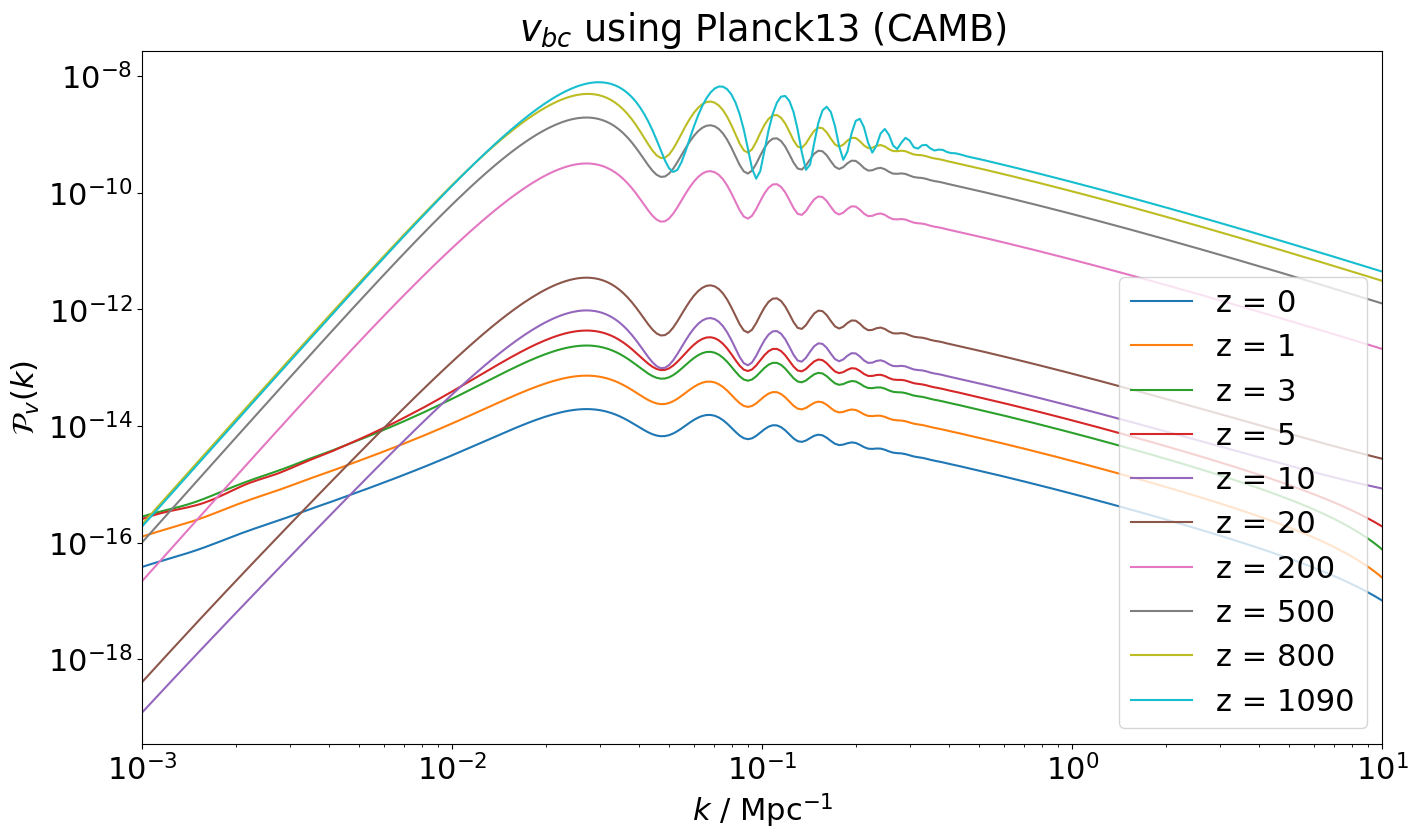
\includegraphics[width=\textwidth]{images/vbc_varied_redshift.png}
         \caption{$v_{bc}$ for various redshifts assuming Planck 2013}
         \label{fig:vbc_varied_redshift}
     \end{subfigure}
     \hfill
     \begin{subfigure}{0.45\textwidth}
         \centering
         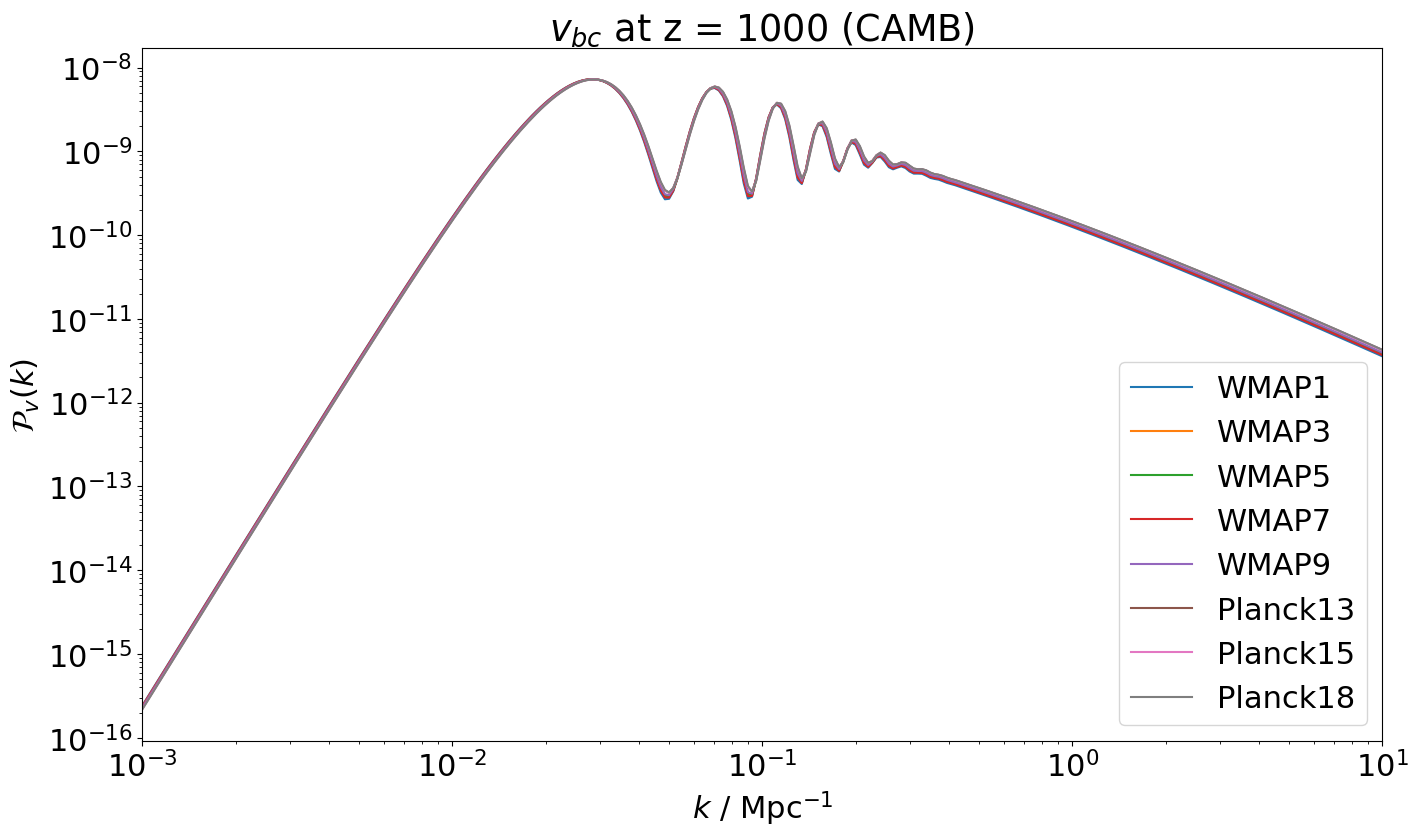
\includegraphics[width=\textwidth]{images/vbc_varied_cosmology.png}
         \caption{$v_{bc}$ for various cosmologies at redshift $z = 1000$}
         \label{fig:vbc_varied_cosmology}
     \end{subfigure}
     \centering
     \begin{subfigure}{0.45\textwidth}
         \centering
         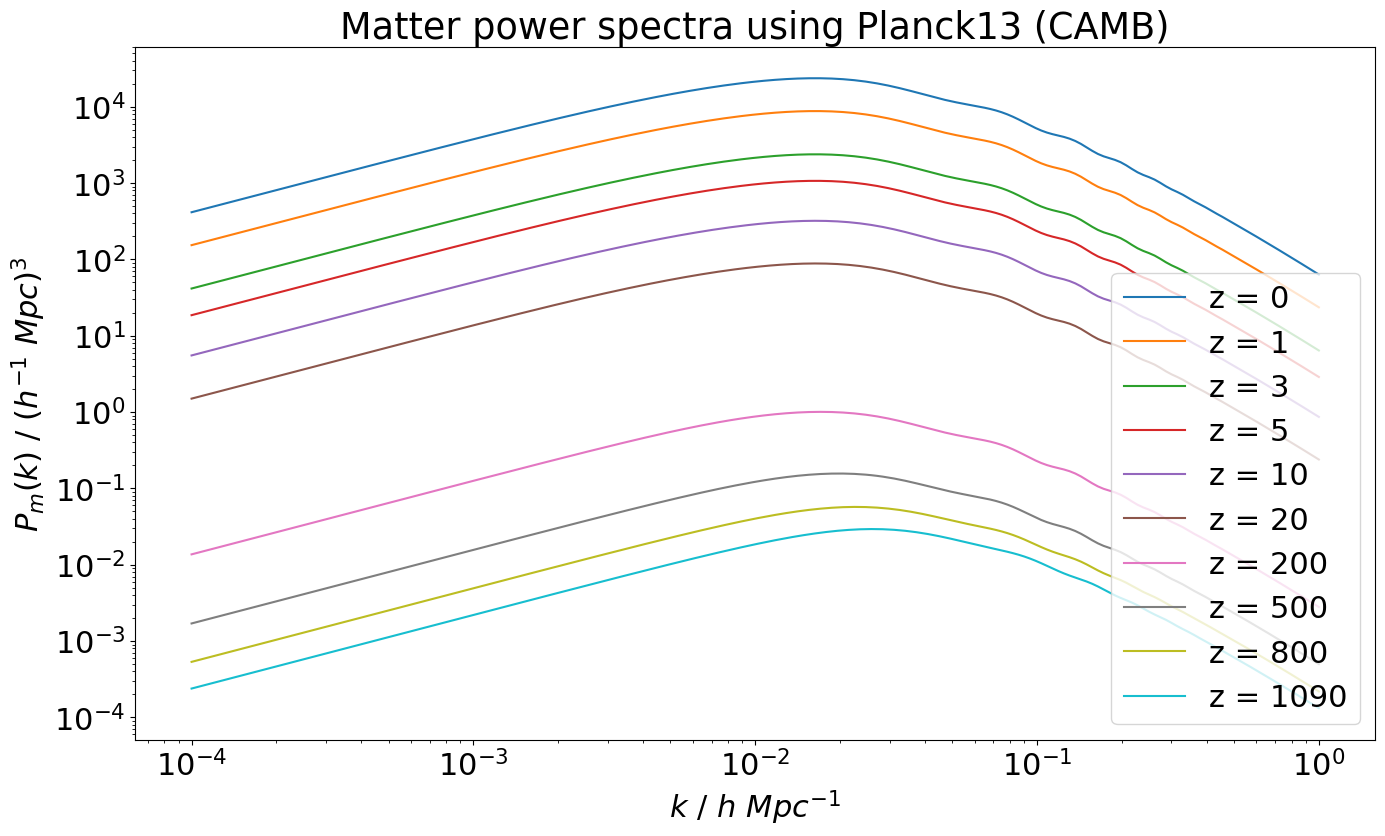
\includegraphics[width=\textwidth]{images/matter_power_spectrum_varied_redshift.png}
         \caption{Matter power spectrum for various redshifts assuming Planck 2013}
         \label{fig:matter_power_spectrum_varied_redshift}
     \end{subfigure}
     \hfill
     \begin{subfigure}{0.45\textwidth}
         \centering
         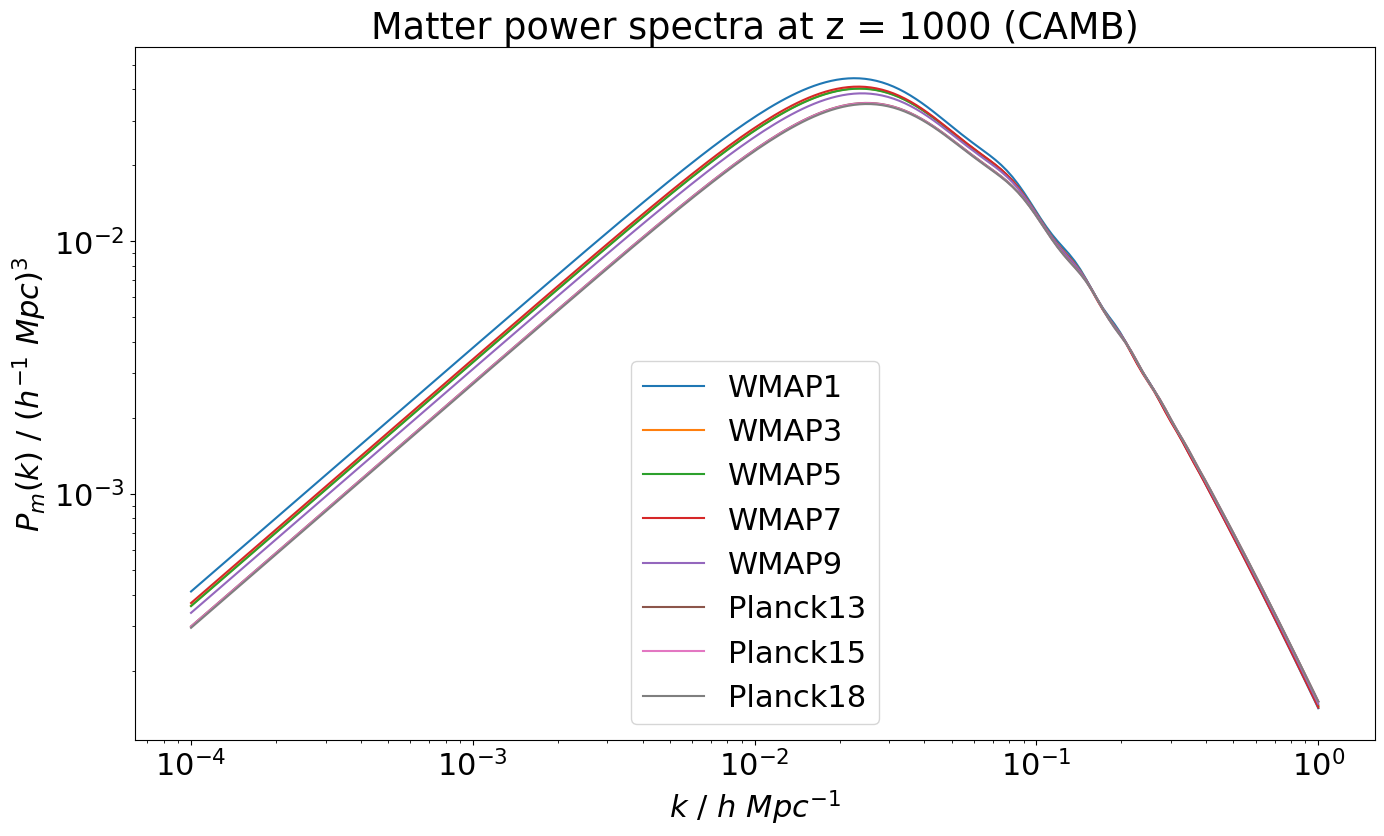
\includegraphics[width=\textwidth]{images/matter_power_spectrum_varied_cosmology.png}
         \caption{Matter power spectrum for various cosmologies at redshift $z = 1000$}
         \label{fig:matter_power_spectrum_varied_cosmology}
     \end{subfigure}
    \caption{Figure \ref{fig:vbc_varied_redshift} shows the $v_{bc}$ power spectrum for the Planck 2013 best fit model (the default cosmology in \code{21cmSPACE}) for various redshifts. Figure \ref{fig:vbc_varied_cosmology} shows the $v_{bc}$ power spectrum for various cosmologies imported from \code{Astropy}. These figures are plotted outputs from \code{CAMB}.}
    \label{fig:camb_output_plots}
\end{figure}


\begin{figure}[!htbp]
     \centering
     \begin{subfigure}{0.45\textwidth}
         \centering
         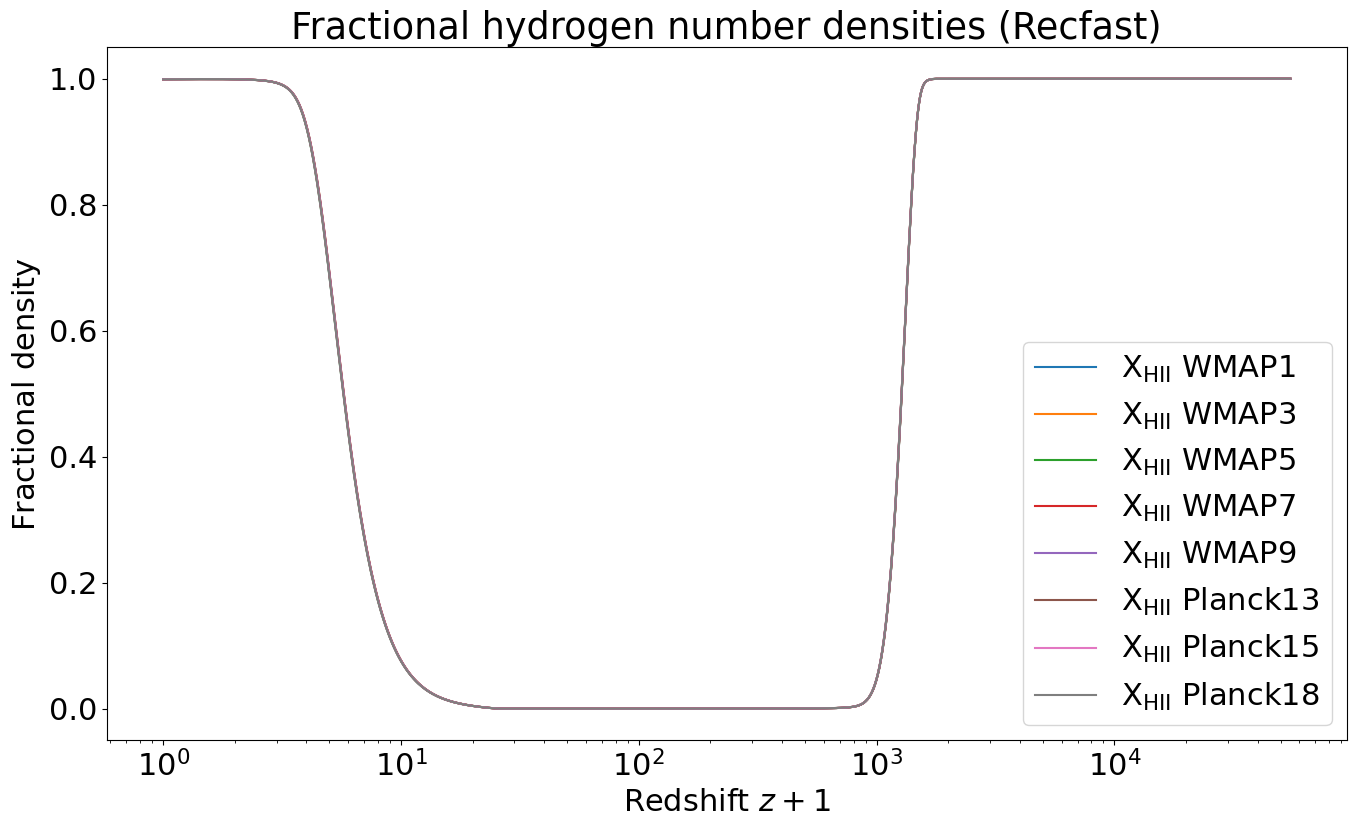
\includegraphics[width=\textwidth]{images/ionized_fraction_varied_cosmology.png}
         \caption{Ionization fraction history of H$_{\text{II}}$ for various cosmologies}
         \label{fig:ionized_fraction}
     \end{subfigure}
     \hfill
     \begin{subfigure}{0.45\textwidth}
         \centering
         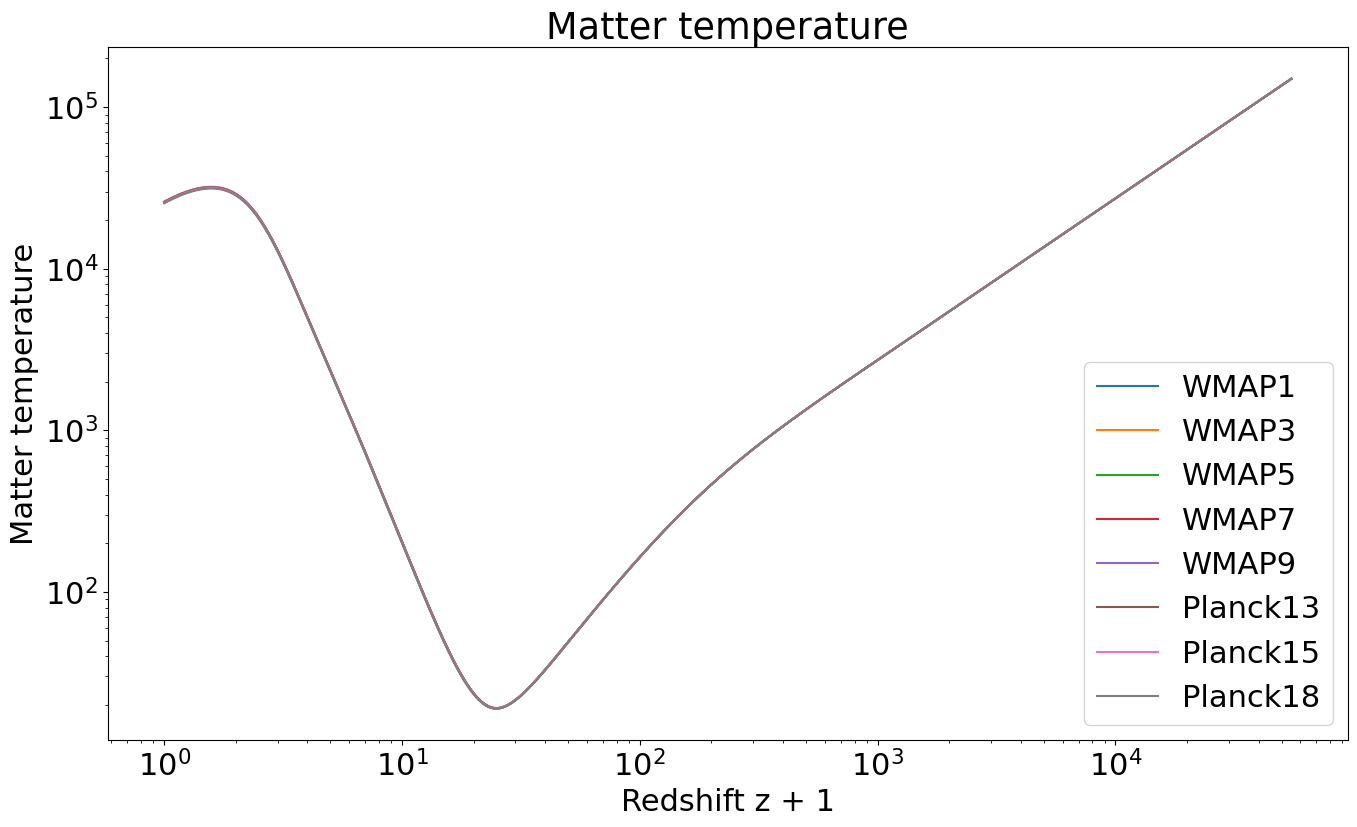
\includegraphics[width=\textwidth]{images/matter_temperature_varied_cosmology.png}
         \caption{Matter temperature history for various cosmologies}
         \label{fig:matter_temperature_varied_cosmology}
     \end{subfigure}
     \caption{Figure \ref{fig:ionized_fraction} shows the ionization history, and Figure \ref{fig:matter_temperature_varied_cosmology} shows the matter temperature history, both for various cosmologies imported from \code{Astropy}. These figures are plotted outputs from \code{Recfast}.}
     \label{fig:recfast_output_plots}
\end{figure}


\begin{figure}[H]
    \centering
    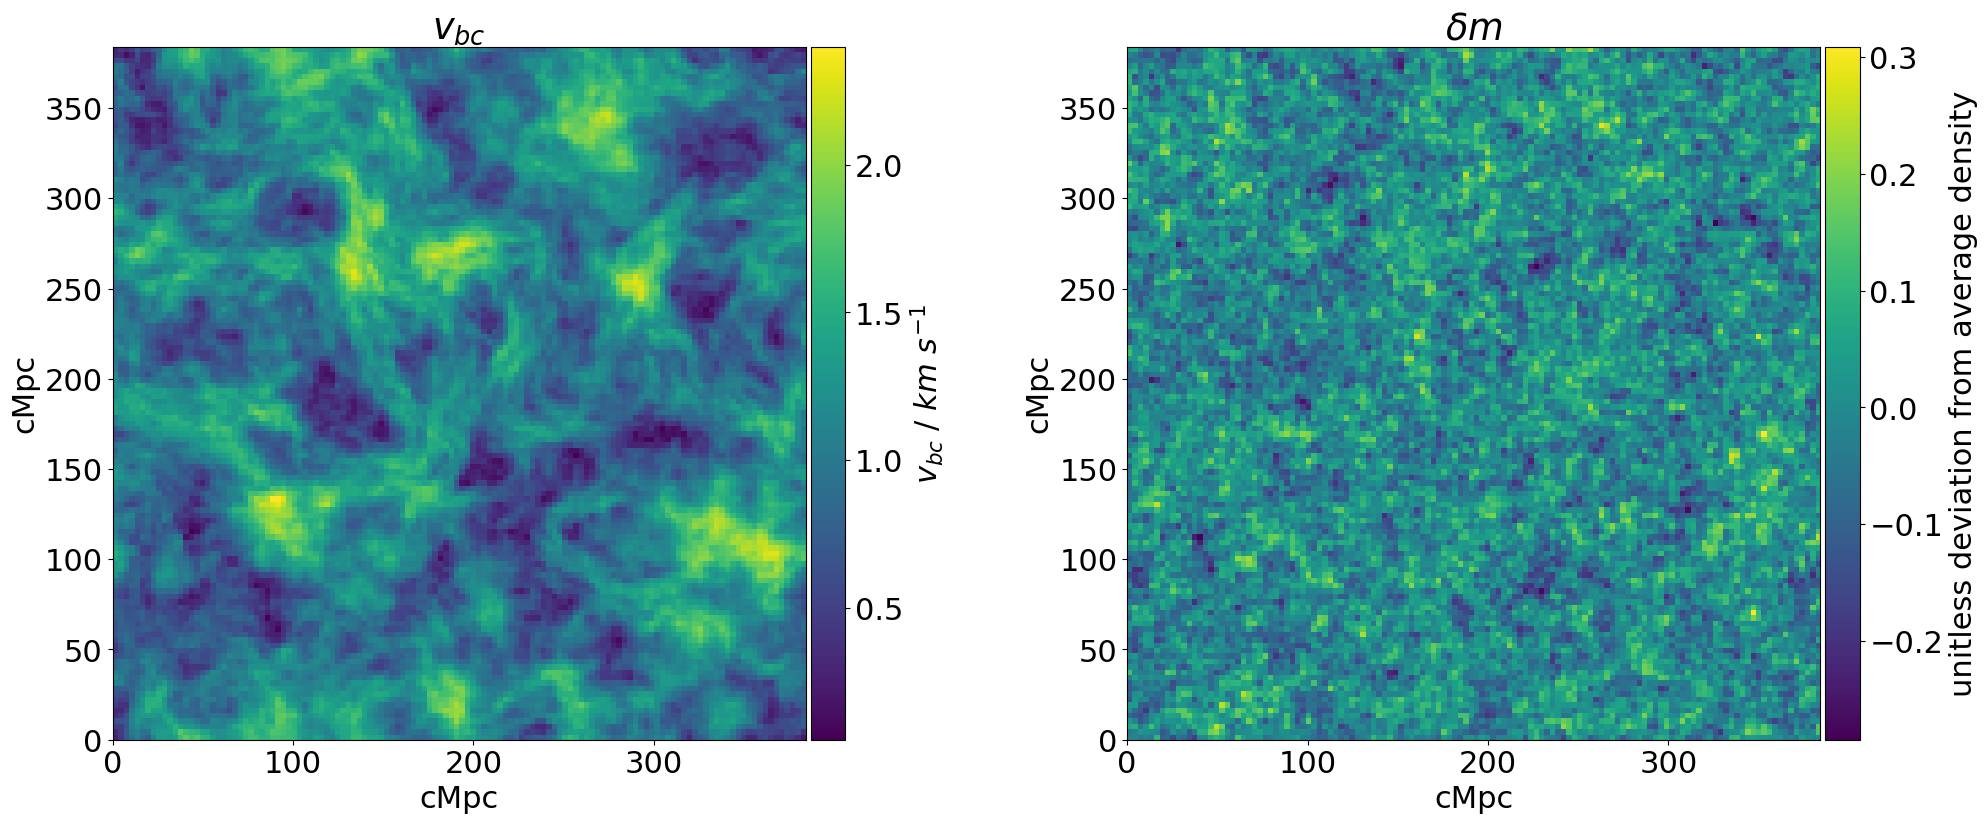
\includegraphics[width=0.9\columnwidth]{images/initial_condition_grid.png}
    \caption{Slices of the 3D initial condition grids as generated from the \code{CAMB} outputs. These specific boxes are generated using the default power spectra contained in \code{21cmSPACE}.}
    \label{fig:initial_condition_grid}
\end{figure}


\section{Upcoming work}

Having invested time learning the usage of \code{CAMB} and \code{Recfast} for generating initial conditions, actual implementation of the initial conditions into the \code{21cmSPACE} MATLAB code by making \code{CAMB} and \code{Recfast} outputs compatible with \code{21cmSPACE} inputs may now follow naturally. As well as this, implementation of variable voxel size will be the next step, followed by rigorous testing of the effects of these changes on the predicted signal. Finally, if time permits, the viability of upscaling these lower-resolution simulations through diffusion models can be explored, possibly recovering the same detail in the final signal at a fraction of the computational cost.

% \begin{acknowledgments}
% K.W. thanks...
% \end{acknowledgments}

\nocite{*}
\printbibliography[title={References}]

\end{document}